\section{Galaxies}\linkdest{gals}

\subsection{Primordial composition and nucleosynthesis}\linkdest{BBN}

\section{MilkyWay}\linkdest{mw}

\begin{frame}{Refs}
The Gaia-ESO Survey: the Galactic Thick to Thin Disc transition
''The Formation and Evolution of the Milky Way: The distribution of the chemicalelements in our galaxy serves as a "fossil record" of its evolutionary history''
''Stellar Populations and the Formation of theMilky Way'' (Majewski)
\end{frame}

\subsection{Via Lattea e gruppo locale. Teorie di formazione galattica}\linkdest{MWoverview}

\begin{frame}{Milky way: thin/thick disk, halo}
\begin{columns}[T]
\begin{column}{0.6\textwidth}
\begin{figure}[!ht]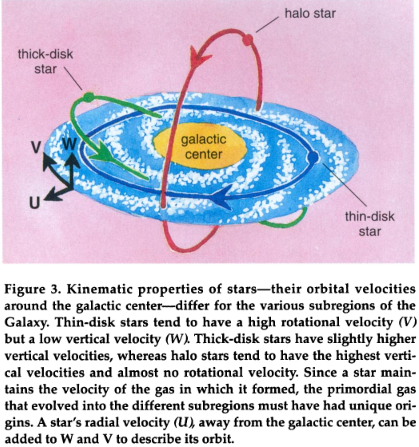
\includegraphics[trim={0cm 0cm 0 0},clip, keepaspectratio,width=0.99\textwidth]{MWcartoon}\label{fig:MWcartoon}\end{figure}
\end{column}
\begin{column}{0.4\textwidth}
Thin: $\exv{z}\approx\SI{300}{\parsec}$, Pop I (many metals absorption lines $Z\approx0.013$)
Thick: $\exv{z}\approx\SI{1000}{\parsec}$, Pop II (absorption line almost. from H: $Z<0.004$)-Int pop I; kinemat. hot, old, $\alpha$-enh metal poor.
Halo: Extreme pop II ($[\alpha/Fe]\approx0.3$)
\end{column}
\end{columns}
\end{frame}

\begin{frame}{Milky way: chemical evolution}
\begin{columns}[T]
\begin{column}{0.6\textwidth}
\begin{figure}[!ht]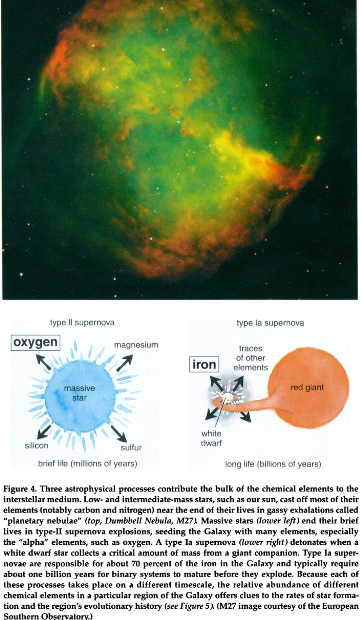
\includegraphics[trim={0cm 0cm 0 0},clip, keepaspectratio,height=0.89\textheight]{PNSNISNII}\label{fig:PNSNISNII}
\end{figure}
\end{column}
\begin{column}{0.4\textwidth}
Massive star: oxigen/$\alpha$-elements (O, Ne, Mg, S, Si, Ca, Ti)
\begin{align*}
&[M/H]=[Fe/H]+\log{(0.694f_{\alpha}+0.306)}\\
&[Fe/H]=\log{(\frac{Z}{X})_*}+1.61
\end{align*}
\end{column}
\end{columns}
\end{frame}

\begin{frame}{Milky way: formation models}
\begin{columns}[T]
\begin{column}{0.4\textwidth}
\begin{figure}[!ht]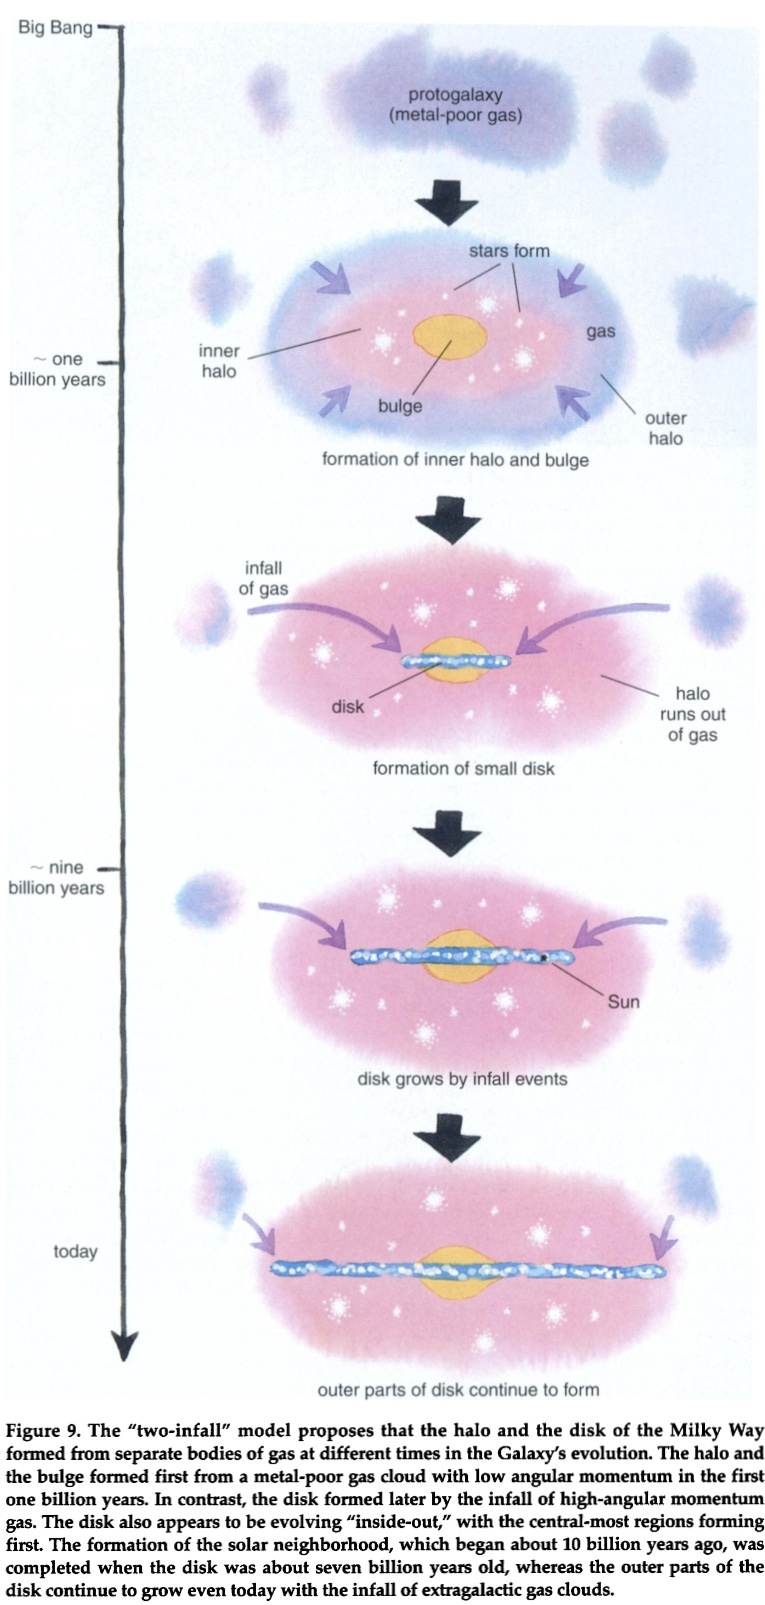
\includegraphics[trim={0cm 0cm 0 0},clip, keepaspectratio,height=0.85\textheight]{MWformation}\label{fig:MWformation}
\end{figure}
\end{column}
\begin{column}{0.6\textwidth}
Two infall model: Low angular momentum materials formed bulge and halo in rapid dissipative collapse (\'a la ELS), mergers with dwarf galaxies (\'a la Searle Zinn) would happened before formation of thin disk: thin disk evolved indipendently from halo from high angular momentum gas, thin disk got thicker in last merger \SI{10}{\giga\year} ago.
Age of thin disk:G dwarf metallicity distribution (Rocha-pinto marciel 1996)
\end{column}
\end{columns}
\end{frame}

\section{Popolazioni stellari}\linkdest{starpop}

\subsection{Problemi osservativi}\linkdest{colormagnitude}

\begin{frame}{Color-Magnitude Diagram}
\begin{columns}[T]
\begin{column}{0.5\textwidth}
\begin{align*}
&M_A=m_A-5\log{d(\si{\parsec})}+5\\
&M_{Bol}=M_{Bol,\odot}-2.5\log{\frac{L}{\lsun{}}}\\
&(A_B)=m_A-m_B
\end{align*}
\end{column}
\begin{column}{0.5\textwidth}
ISM extintion $f_{\lambda}=f_ {\lambda,0}\exp{-\tau_{\lambda}}$, $\tau_{\lambda}$ ISM optical depth $\propto\invers{\lambda}$:
\begin{equation*}
m_A=-2.5\log{(\frac{\int_{\lambda_1}^{\lambda_2}f_{\lambda}10\expy{-0.47A_{\lambda}}S_{\lambda}\,d\lambda}{\int_{\lambda_1}^{\lambda_2}f_{\lambda}^0S_{\lambda}\,d\lambda})}
\end{equation*}
\end{column}
\end{columns}
\end{frame}


\subsection{Popolazioni semplici}\linkdest{spcpx}

\begin{frame}{Empirical IMF}
\begin{align*}
&dn=CM\expy{-x}\,dM\\
&C=(2-x)\frac{M_t}{M_u\expy{2-x}-M_l\expy{2-x}}\\
&C=\frac{M_t}{\ln(\frac{M_u}{M_l})}
\end{align*}
\end{frame}

\begin{frame}{SSP: theoretical isochrones}
\begin{columns}[T]
\begin{column}{0.4\textwidth}
\begin{figure}[!ht]
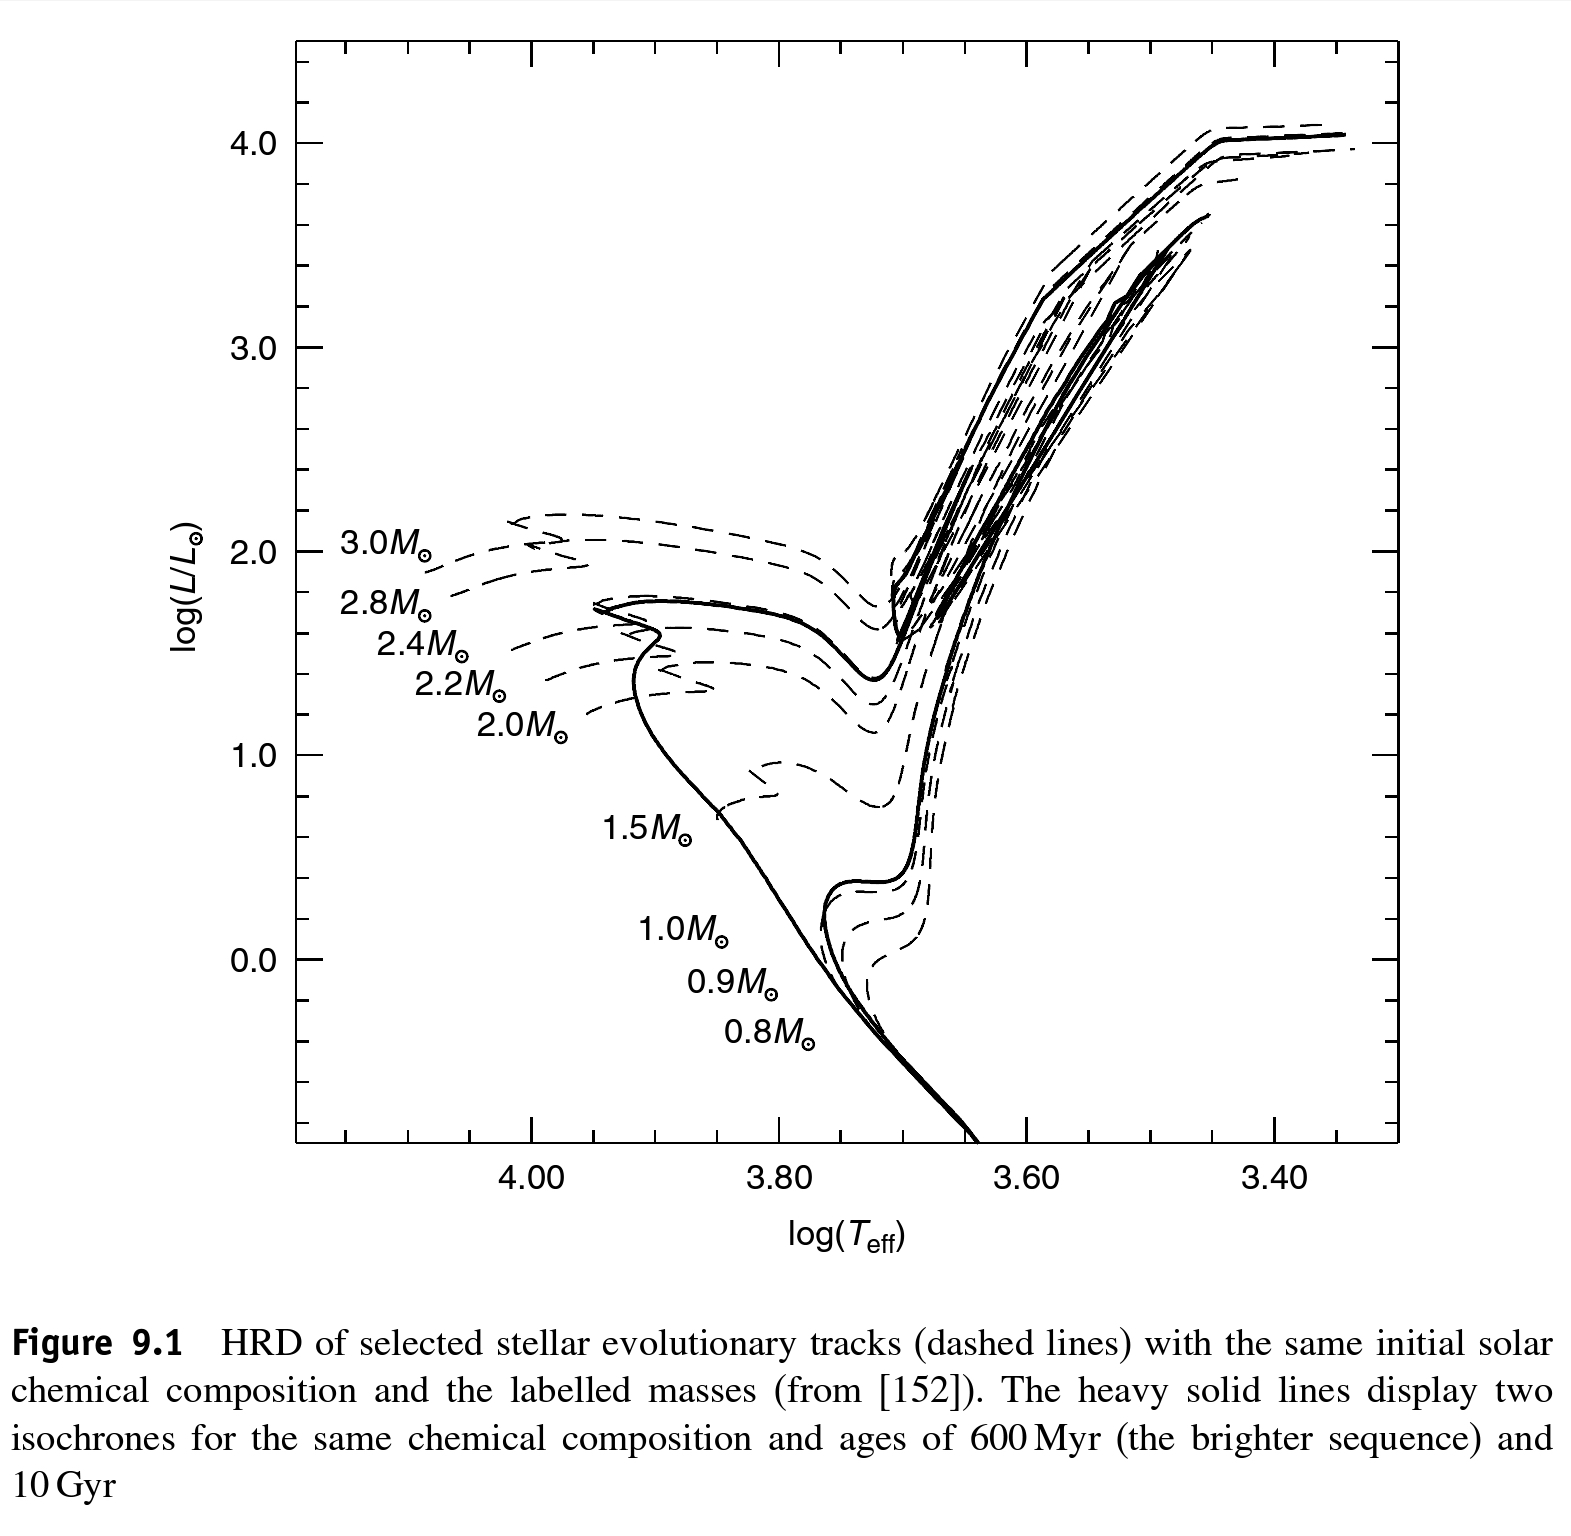
\includegraphics[trim={0cm 0cm 0 0},clip, keepaspectratio,height=0.4\textheight]{isochr}\label{fig:isochr}
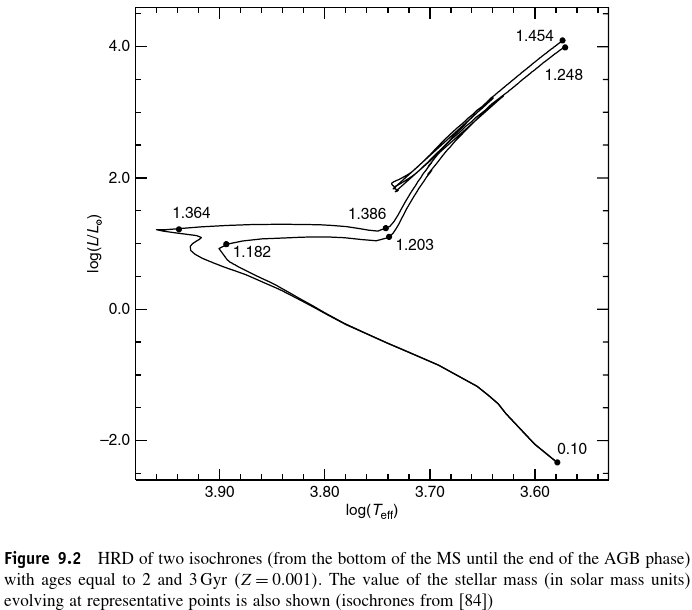
\includegraphics[trim={0cm 0cm 0 0},clip, keepaspectratio,height=0.4\textheight]{SSP-isoMSAGB}\label{fig:SSP-isoMSAGB}
\end{figure}
\end{column}
\begin{column}{0.6\textwidth}
\begin{itemize}
\item Object born at same time in burst of negligible duration with same initial composition; theoretical CMD of SSP is an isochrone at given age.
\item s coordinata lungo isocrona: $\TDy{s}{M}|_t=-\TDy{t}{M}|_s\TDy{s}{t}|_M$ - if rightside close to zero mass evolving in that particular phase is constant
\end{itemize}
\end{column}
\end{columns}
\end{frame}

\begin{frame}{Old SSP: globular cluster and halo star}
\begin{columns}[T]
\begin{column}{0.4\textwidth}
		\begin{figure}[!ht]
		\includegraphics[trim={0cm 0cm 0 0},clip, keepaspectratio,width=0.99\textwidth]{SSP-iso10GyrHB}\label{fig:SSP-iso10GyrHB}
		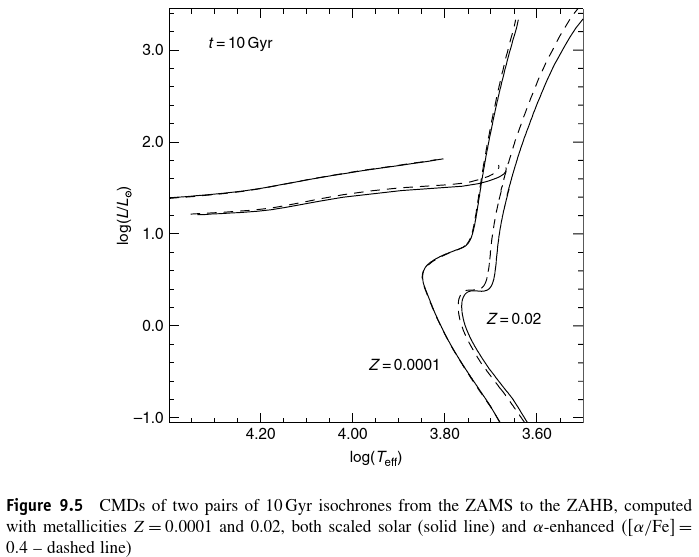
\includegraphics[trim={0cm 0cm 0 0},clip, keepaspectratio,width=0.99\textwidth]{SSP-CMDalpha}\label{fig:SSP-CMDalpha}
		\end{figure}
\end{column}
\begin{column}{0.6\textwidth}
		\begin{itemize}
		\item Fig 9.3 shows a \SI{10}{\giga\year} isochrone for metal-poor chem comp typical of globular cluster
		\item $[\alpha/Fe]=0.4$ tipical MW halo - at low Z isochrones are identical - scaled solar are redder and fainter at given Z when traslated to CMD
		\end{itemize}
\end{column}
\end{columns}
\end{frame}

\begin{frame}{Old SSP: effect of ages and Zs}
\begin{columns}[T]
	\begin{column}{0.4\textwidth}
		\begin{figure}[!ht]
		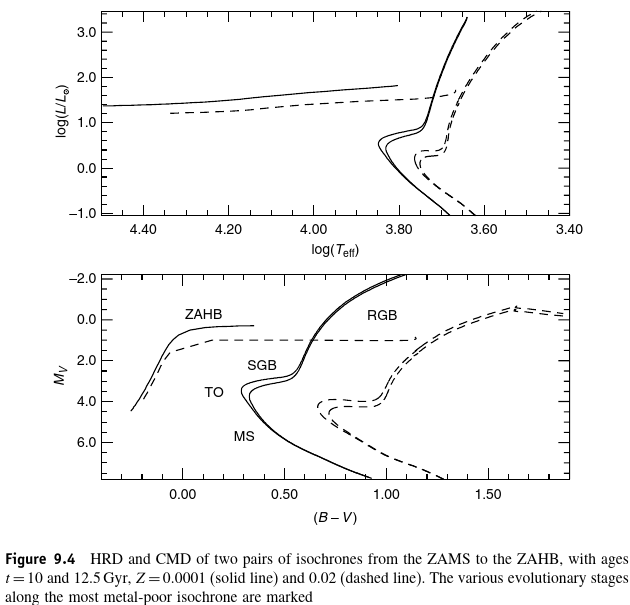
\includegraphics[trim={0cm 0cm 0 0},clip, keepaspectratio,width=0.99\textwidth]{SSP-HDRCMDZpoorMSHB}\label{fig:SSP-HDRCMDZpoorMSHB}
		\end{figure}
	\end{column}
	\begin{column}{0.6\textwidth}
		\begin{itemize}
			\item Props of fig 9.4: lower-MS (starting from \SI{2}{\mag} below TO) and RGB unaffected by age but sensitive to Z: lower MS have very long $\tau$ and are still on ZAMS - increasing t-iso lower $M_*$ are at TO hence \xdiminuisce{L_{TO}} - \xaumenta{Z} \xdiminuisce{L_{MS}} compensate the fact that higher Z SSP have higher $M_*$ at TO; RGB depends weakly on $M_*$ and strongly on Z which strongly affect T of RGB; brightness of ZAHB unaffected by age but deps on Z - mostly deps on $M_{cHe}$ at He flash: \xaumenta{Z}, \xdiminuisce{M{cHe}}, age doesn't affect He-core mass for evolving stars RGB stars older than \SI{4}{\giga\year} ($M_*\leq1.2-1.3\msun$);
		\end{itemize}
	\end{column}
\end{columns}
\end{frame}

\begin{frame}{Popolazioni in galassie esterne}
star formation history; popo non risolte semplici e complesse
\end{frame}

\subsection{Indicatori d'et\'a}\linkdest{ageindicator}

\begin{frame}{indicatori di et\'a}
Turn-off/overall contraction: Isocrone di ammassi giovani/vecchi; metodo orizzontale e vertical per ammassi antichi; Lithium depletion boundary per datazione di ammassi giovani
\end{frame}

\begin{frame}{Indicatori di et\'a: metodo verticale}
\begin{columns}[T]
	\begin{column}{0.5\textwidth}
		\begin{figure}[!ht]
			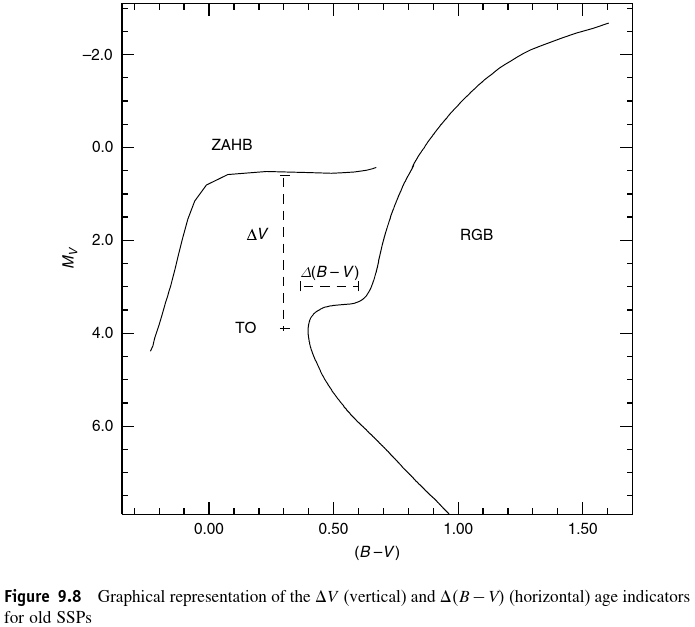
\includegraphics[trim={0cm 0cm 0 0},clip, keepaspectratio,width=0.99\textwidth]{SSP-agevert}\label{fig:SSP-agevert}
		\end{figure}
	\end{column}
	\begin{column}{0.5\textwidth}
		\begin{itemize}
		\item Comparison between observed and theretical $\Delta V=V_{TO}-V_{ZAHB}$ difference between TO point and ZAHB point at instability strip region around $\log(T_e)\approx3.85$ ($(B-V\approx0.3)$)
		\item ZAHB is unaffected by age: changes of age at given $Fe/H$ changes $\Delta V$ through change in TO-brightness
		\end{itemize}
	\end{column}
\end{columns}
\end{frame}

\subsection{Indicatori di distanza}\linkdest{distanceindicator}

\begin{frame}{Distanza ammassi}
main sequence fitting
tip rgb
ZAHB
clump elio
RR lyrae
cefeidi
\end{frame}

\subsection{Popolazioni stellari composite (CSP)}

\begin{frame}{Complex Stellar Population}
    
\end{frame}



\begin{frame}{Indicatori di He (e Z??)}
??
\end{frame}
